%&template
\documentclass{article}
\usepackage{src/template}

\endofdump
\usepackage{minted}

\date{2025 -- 11 -- 09}
\useTemplate[NPA, Exercise=3]
\title{NPA -- Exercise 3}


\begin{document}
\maketitle

    \section{}
            
        \subsection{}
            The SDN setup can be divided into two planes: the data plane, consisting of the switches in the network, and the control plane, consisting of first the SDN controller and second the network-control applications.
            In general, the SDN controller maintains network state information provided by the switches, such as link state information, statistics and flow tables. Different higher level functions such as path-planning or load-balancing can be found in the network-control applications.
            Upon detecting a change on a port (e.g. Link is down), the SDN controller will be informed of the change with a message. 

            In order to detect an overloaded in a server, the amount of traffic has to be monitored as well. This could be done at all times (regular interval of informing the SDN about traffic statistics) or when the amount of traffic exceeds a certain threshold. 
            Upon receiving the message at the SDN, this information needs to be passed to the network-control app responsible for load balancing. This app, in turn, needs to recompute routes such that the traffic will be more balanced. This will lead to a recomputation of the flow-tables. 

            This change will then be propageted down the stack, first to the SDN and afterwards to the switches on the data plane.
            
        \subsection{}
            A \enquote{Load Balancing Application} would use the Northbound SDN interface to communicate with the SDN controller. 

            The flow rule the SDN would send is to match the Destination IP of the overloaded server and forward it to a server that is not overloaded.

            An example scenario can be seen in \ref{fig:ex03_q01_b}. Assume Server A (10.42.0.41) is the overloaded server and Server A and B (10.42.0.42) have the same functionality. SW11 and SW12 are connected to a uplink, where requests can originate from.

            Then, to enforce load balancing, the SDN would send a rule to SW11 to match the destination IP 10.42.0.41 and forward it instead to 10.42.0.42, despite the path SW11$\to$SW21 having a higher cost than SW11$\to$SW12.
            \begin{figure}[H]
                \centering
                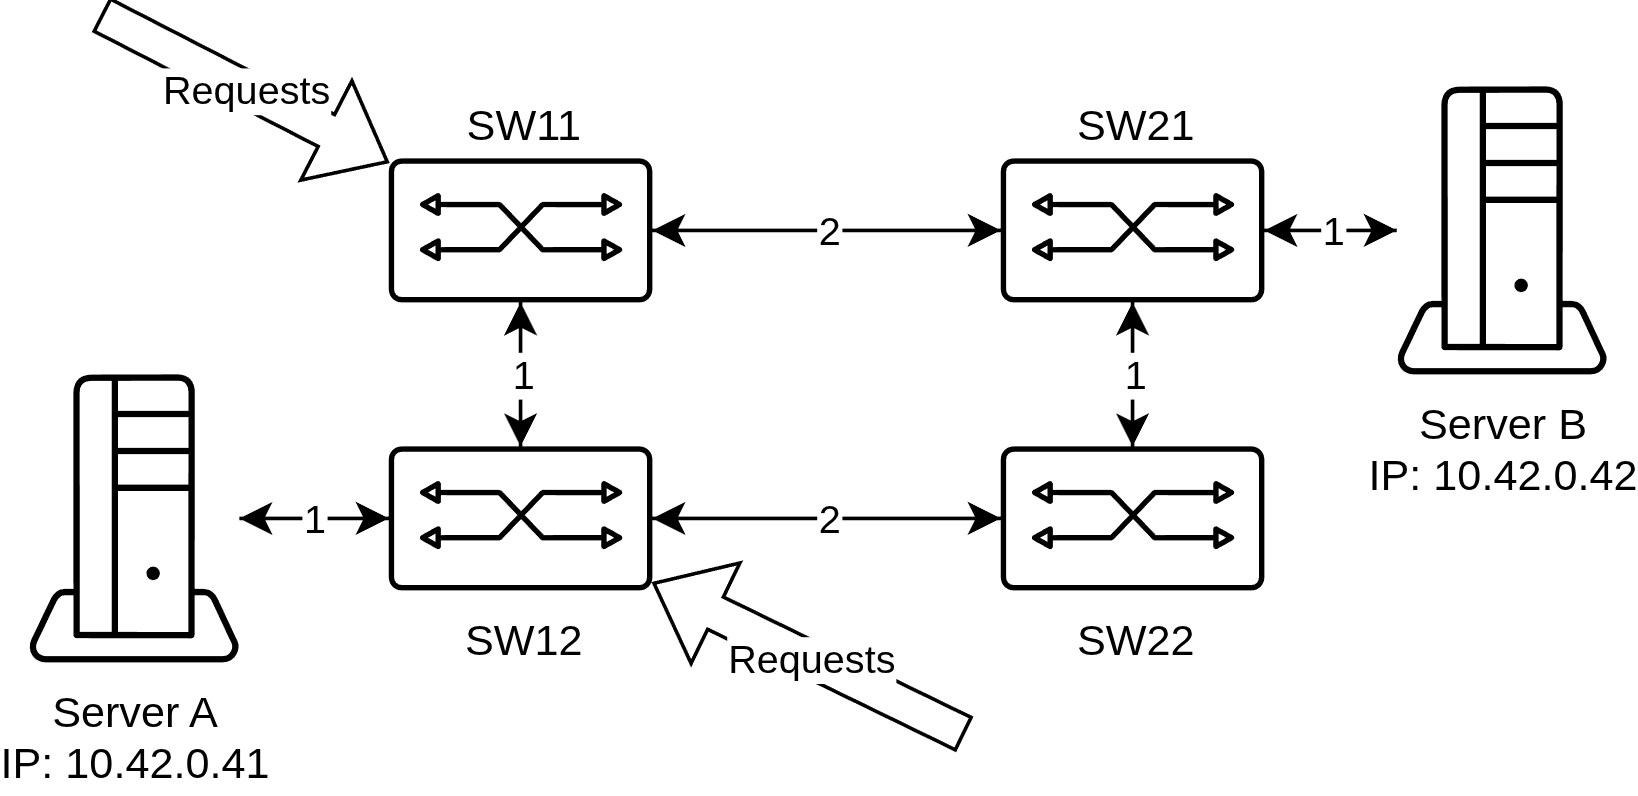
\includegraphics[width=0.5\linewidth]{images/ex03-q01-b.png}
                \caption{Example Network for Load Balancing}
                \label{fig:ex03_q01_b}
            \end{figure}
            
    
    
    \newpage
    \section{}
    \subsection{}

    The graphical representation of \texttt{dumbbell\_topo.py} looks like:
    
    \begin{center}
        \begin{figure}[H]
            \centering
            %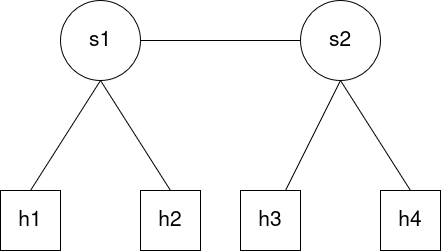
\includegraphics{images/homework03-exercise02a.png}
            \begin{tikzpicture}[
                host/.style={rectangle, draw, thick, minimum size=10mm, fill=blue!15},
                switch/.style={circle, draw, thick, minimum width=15mm, minimum height=10mm, fill=orange!20},
                con1/.style={line width=1},
                con2/.style={line width=1},
                con3/.style={line width=1, decoration={random steps,segment length=2mm}, decorate},
                >=latex
                ]
                    % Switches
                    \node[switch] (s1) {s1};
                    \node[switch, right=3cm of s1] (s2) {s2};

                    % Hosts
                    \node[host, left=2cm of s1, yshift=10mm] (h1) {h1};
                    \node[host, left=2cm of s1, yshift=-10mm] (h2) {h2};
                    \node[host, right=2cm of s2, yshift=10mm] (h3) {h3};
                    \node[host, right=2cm of s2, yshift=-10mm] (h4) {h4};

                    % Connections
                    \draw[con2] (h1) -- (s1);
                    \draw[con2] (h2) -- (s1);
                    \draw[con1] (s1) -- (s2);
                    \draw[con2] (s2) -- (h3);
                    \draw[con2] (s2) -- (h4);

            \end{tikzpicture}
            \caption{Dumbbell topology}
            \label{fig:placeholder}
        \end{figure}
    \end{center}
    
    \subsection{}

    We extend the program \texttt{mac-learning.py} to include the Mac Learning algorithm presented in the lecture. We modify the function \texttt{\_packet\_in\_handler()} as follows:
    
    \begin{minted}[escapeinside=@@,breaklines]{py}
    def _packet_in_handler(self, ev):
        msg = ev.msg
        datapath = msg.datapath
        switch_id = datapath.id
        ofproto = datapath.ofproto
        parser = datapath.ofproto_parser

        in_port = msg.match['in_port']

        pkt = packet.Packet(msg.data)
        ether_info = pkt.get_protocol(ethernet.ethernet)

        # debug output
        # print(f"Switch {switch_id} received a packet on port {in_port} with src MAC {ether_info.src} and dst MAC {ether_info.dst}")

        # flood
        actions_flood = [parser.OFPActionOutput(ofproto.OFPP_FLOOD)]
        match_flood = parser.OFPMatch(in_port=in_port)

        out = parser.OFPPacketOut(
            datapath=datapath,
            buffer_id=ofproto.OFP_NO_BUFFER,
            match=match_flood,
            actions=actions_flood,
            data=msg.data
        )
        datapath.send_msg(out)

        # learn MAC adress to avoid flooding next time
        match_learn = parser.OFPMatch(eth_dst=ether_info.src)
        actions_learn = [parser.OFPActionOutput(in_port)]
        self.add_flow(datapath, actions=actions_learn, priority=1, match=match_learn, timeout=20)
        # We choose idle_timeout and not hard_timeout, because it seems to be more what the exercise wants.
        # Adding a hard timeout would remove the entry after a fixed time, regardless of activity.
        
    \end{minted}

    
    We execute our created rules on the topology shown in \ref{fig:placeholder} and first demonstrate that the switches have no rules defined. After pinging of all hosts, the routes were learned based on the MAC addresses, and as described in the exercise, the rules are discarded after 20 seconds.


    \begin{minted}[escapeinside=@@,breaklines]{sh}
vagrant@mininet:/vagrant$ sudo mn --custom dumbbell_topo.py --topo dumbbell --controller=remote
    *** Creating network
    *** Adding controller
    Unable to contact the remote controller at 127.0.0.1:6653
    Unable to contact the remote controller at 127.0.0.1:6633
    Setting remote controller to 127.0.0.1:6653
    *** Adding hosts:
    h1 h2 h3 h4 
    *** Adding switches:
    s1 s2 
    *** Adding links:
    (h1, s1) (h2, s1) (h3, s2) (h4, s2) (s1, s2) 
    *** Configuring hosts
    h1 h2 h3 h4 
    *** Starting controller
    c0 
    *** Starting 2 switches
    s1 s2 ...
    *** Starting CLI:
mininet> sh ovs-ofctl dump-flows s1
    cookie=0x0, duration=0.912s, table=0, n_packets=0, n_bytes=0, priority=0 actions=CONTROLLER:65535
mininet> sh ovs-ofctl dump-flows s2
    cookie=0x0, duration=3.044s, table=0, n_packets=0, n_bytes=0, priority=0 actions=CONTROLLER:65535
mininet> pingall
    *** Ping: testing ping reachability
    h1 -> h2 h3 h4 
    h2 -> h1 h3 h4 
    h3 -> h1 h2 h4 
    h4 -> h1 h2 h3 
    *** Results: 0% dropped (12/12 received)
mininet> sh ovs-ofctl dump-flows s1
    cookie=0x0, duration=4.379s, table=0, n_packets=1, n_bytes=42, idle_timeout=20, priority=1,dl_dst=4a:c4:5e:29:4c:f4 actions=output:"s1-eth3"
    cookie=0x0, duration=4.372s, table=0, n_packets=7, n_bytes=574, idle_timeout=20, priority=1,dl_dst=6e:e9:1a:4a:bf:50 actions=output:"s1-eth2"
    cookie=0x0, duration=2.519s, table=0, n_packets=9, n_bytes=714, idle_timeout=20, priority=1,dl_dst=b6:bf:1a:81:94:3e actions=output:"s1-eth1"
    cookie=0x0, duration=1.775s, table=0, n_packets=0, n_bytes=0, idle_timeout=20, priority=1,dl_dst=d6:05:46:8f:6b:a0 actions=output:"s1-eth3"
    cookie=0x0, duration=13.984s, table=0, n_packets=17, n_bytes=1274, priority=0 actions=CONTROLLER:65535
mininet> sh ovs-ofctl dump-flows s2
    cookie=0x0, duration=4.924s, table=0, n_packets=8, n_bytes=560, idle_timeout=20, priority=1,dl_dst=b6:bf:1a:81:94:3e actions=output:"s2-eth3"
    cookie=0x0, duration=4.184s, table=0, n_packets=7, n_bytes=518, idle_timeout=20, priority=1,dl_dst=d6:05:46:8f:6b:a0 actions=output:"s2-eth2"
    cookie=0x0, duration=2.115s, table=0, n_packets=5, n_bytes=322, idle_timeout=20, priority=1,dl_dst=4a:c4:5e:29:4c:f4 actions=output:"s2-eth1"
    cookie=0x0, duration=0.095s, table=0, n_packets=0, n_bytes=0, idle_timeout=20, priority=1,dl_dst=5e:ef:2f:a3:64:fb actions=output:"s2-eth3"
    cookie=0x0, duration=0.095s, table=0, n_packets=9, n_bytes=658, idle_timeout=20, priority=1,dl_dst=6e:e9:1a:4a:bf:50 actions=output:"s2-eth3"
    cookie=0x0, duration=16.390s, table=0, n_packets=19, n_bytes=1330, priority=0 actions=CONTROLLER:65535
mininet> sh ovs-ofctl dump-flows s2
    cookie=0x0, duration=88.282s, table=0, n_packets=24, n_bytes=1680, priority=0 actions=CONTROLLER:65535
mininet> sh ovs-ofctl dump-flows s1
    cookie=0x0, duration=90.990s, table=0, n_packets=25, n_bytes=1834, priority=0 actions=CONTROLLER:65535

    \end{minted}

    
    
\end{document}